\documentclass[conference]{IEEEtran}

% ---------------------------------------------------------------
% Packages
% ---------------------------------------------------------------
\usepackage{cite}
\usepackage{amsmath,amssymb}
\usepackage{graphicx}
\usepackage{url}
\usepackage{xcolor}
\usepackage{booktabs}   % \toprule / \midrule / \bottomrule
\usepackage{listings}   % code listings

% ---------------------------------------------------------------
% Title / Authors
% ---------------------------------------------------------------
\title{Replication Study of Web-Based PLC Malware: Firmware Analysis, Service Worker Resurrection, and Behavioral Anomaly Detection}

\author{
  \IEEEauthorblockN{Hojune Kim}
  \IEEEauthorblockA{School of Computing\\
    Korea Advanced Institute of Science and Technology, Daejeon, Republic of Korea\\
    {hojunekim}@kaist.ac.kr}
}

\begin{document}
\maketitle

\lstset{
  basicstyle=\ttfamily\footnotesize,
  breaklines=true,
  frame=single,
  backgroundcolor=\color{gray!8},
}

% ---------------------------------------------------------------
% Abstract
% ---------------------------------------------------------------
\begin{abstract}
This is a replication study of ``Compromising Industrial Processes using Web-Based PLC Malware'' (Pickern et al., NDSS 2024), which proposed IronSpider --- a web-based malware that persists within the web interface of modern programmable logic controllers (PLCs) and bypasses factory reset via a Service Worker resurrection scheme.  
%
This study reproduces the paper's firmware complexity analysis (E1) across four WAGO 750-8XXX firmware versions ranging from 2019 to 2023, conducts additional qualitative analysis on firmware JavaScript API features, and created a standalone browser testbed for the full six-step resurrection cycle (E4) including survival of hardware replacement.
%
Furthermore, this study implements the three key attack capabilities inspired by IronSpider --- sensor spoofing, alarm supression, and actuator manipulation --- by manual malware injection, which is analogous to CVE-driven code injection in the paper.
%
Finally, this study strives to solve the paper's open detection problem of web-based PLC malware by implementing a server-side runtime detector inside OpenPLC's Flask webserver. Tier~1 alert shows zero false positive over five minutes of normal operation by setting up detection logic for two browser-generated request headers: \texttt{Sec-Fetch-Dest: empty} and a \texttt{Referer} originating from a \texttt{.js} context. The detection technique is evaluated with three evasion methods, two of which defeat Tier~1 with suggestions on countermeasures. 
\end{abstract}

\begin{IEEEkeywords}
PLC malware, industrial control systems, Service Worker, web security,
behavioral detection, ICS
\end{IEEEkeywords}

% ---------------------------------------------------------------
% I. Introduction
% ---------------------------------------------------------------
\section{Introduction}

Industrial control systems (ICSs) are the backbone of critical infrastructures such as water treatment plant, power grids, and manufacturing factories. They have been considered to be free of web-based attack vectors, due to its traditional isolation from the open Internet. However, this assumption has become obsolete as modern PLCs gradually provide more support for browser-based human-machine interfaces (HMIs) and embedded web server, which allow for remote system monitoring and configuration. The boundary between operational technology (OT) and information technology (IT) is fading, and ICSs are now open to web-based attack.

Pickren et al.~\cite{ironspider2024} proposed IronSpider, a
web-based PLC malware (WB PLC malware) that hinders the system entirely within the
operator's browser. Unlike traditional PLC malware (e.g., Stuxnet~\cite{stuxnet}, HARVEY~\cite{}), IronSpider does not require prior knowledge of firmware or kernel exploits; it only utilises browser APIs to control the system as if it were a legitimate human operator. The paper demonstrates key attack capabilities such as sensor spoofing and actuator manipulation, along with a Service Worker (SW) resurrection mechanism that revives the malware after factory reset, surviving even hardware replacement. Another key finding is that four established JavaScript malware detectors (Cujo, Zozzle, JaSt, JStap) all failed to categorise IronSpider as malicious, since the malware does not contain any aggressive or syntactically suspicious code patterns \cite{ironspider2024}.

This study contains a structured replication study conducted over
19 days with four contributions:
\begin{enumerate}
  \item \textbf{Firmware growth analysis (E1).} This study replicates the paper's SLOC and cyclomatic complexity measurements on four WAGO firmware versions (two from the paper, two intermediate chosen by this study). Also, we extend the analysis qualitatively by observing any change in JavaScript API surface between versions. 
  \item \textbf{Service Worker resurrection testbed (E4).} 
      This study builds a standalone Node.js/HTTPS testbed showing the full six-step resurrection process of WB PLC malware and demonstrate hardware replacement survival and the 24-hour cache limit of SWs.

  \item \textbf{OpenPLC capability demonstration.} 
      This study implements the three key attack capabilities of IronSpider on OpenPLC via manual payload injection --- an adaptation which preserves the attack characteristics while acknowledging that CVE-driven code injection in OpenPLC is not feasible, unlike in the original WAGO case.

  \item \textbf{Behavioral anomaly detection.} This study implements a server-side detector as a component of OpenPLC's Flask webserver, addressing the detection gap stated in the paper. The Tier~1 heuristic makes use of browser-generated Fetch metadata headers to detect SW constantly checking for the malware's presence, while keeping the number of false positives to zero.
\end{enumerate}

The remainder of the paper is organised as follows.
Section~\ref{sec:background} covers background on ICS architecture,
WB PLC malware, and the OpenPLC browser APIs exploited.
Section~\ref{sec:methodology} describes the test environment and experimental
adaptations.
Sections~\ref{sec:e1}--\ref{sec:detection} present results.
Section~\ref{sec:discussion} discusses implications and limitations.
Section~\ref{sec:conclusion} concludes.

% ---------------------------------------------------------------
% II. Background
% ---------------------------------------------------------------
\section{Background}
\label{sec:background}

\subsection{ICS Architecture and the PERA Model}

Industrial control systems typically adopts the Purdue Enterprise Reference Architecture (PERA) model, which categorises assets into five levels: Level~0 (field devices and sensors),
Level~1 (basic control including PLCs, RTUs), Level~2 (supervisory control including
HMIs, SCADA), Level~3 (site operations network), and Level~4 (enterprise
network). WB PLC malware places itself entirely within the OT boundary (Level~2), spoofing HMI values and controlling actuators on its own.

\subsection{Web-Based PLC Malware vs.\ Traditional PLC Malware}

Traditional PLC malware (e.g., Stuxnet~\cite{stuxnet},
Harvey~\cite{harvey2017}) often requires specific knowledge about the victim's instruction set and PLC firmware. In comparison, WB PLC malware only exploits the victim browser's web API for controlling the underlying PLC, imitating the legitimate human operator behind the HMI.

\subsection{Service Workers and the Resurrection Mechanism}

A Service Worker (SW) is a JavaScript file that the browser registers as a persistent background proxy for a web origin~\cite{w3c-sw}. Key properties that IronSpider exploits:

\begin{itemize}
  \item \textbf{Persistence.}
        SW registrations are stored on the browser's side; deleting the injected SW file from the server does not remove the registered SW.
  \item \textbf{CacheStorage.} SWs can store data in
        \texttt{CacheStorage}, which persists without explicit user action or storage pressure.
  \item \textbf{Same-origin fetch privilege.} 
        A SW registered on the PLC's web context can call any same-origin web API without cross-origin resourcce sharing (CORS) restriction, exploiting the operator's authenticated session.
  \item \textbf{DOM bypass via \texttt{respondWith}.} 
        SWs do not have direct DOM access, but they can intercept HTTP responses and inject arbitrary JavaScript code. The injected code runs in the page context with full DOM access.
\end{itemize}

The resurrection cycle (Fig.~4 of~\cite{ironspider2024}) works as follows: after initial infection, the SW caches the malware payload in CacheStorage. If a factory reset occurs, the SW detects the 404 after trying to GET the malware. It then retrieves the cached copy, and re-uploads it using the same CVE chain exploited to inject the malware.

\subsection{Static JS Malware Detection and Its Limits}

The paper attempted at detecting IronSpider using four static JavaScript analysers: Cujo~\cite{cujo}, Zozzle~\cite{zozzle}, JaSt~\cite{jast}, and JStap~\cite{jstap}. All four classified IronSpider as benign, since it lacks aggressive indicators such as mining cryptocurrency in WebAssembly.

% ---------------------------------------------------------------
% III. Methodology
% ---------------------------------------------------------------
\section{Methodology}
\label{sec:methodology}

\subsection{Testbed Overview}

The study uses two separate test environments:

\begin{enumerate}
  \item \textbf{E1 firmware analysis.} WAGO 750-8XXX firware images v3.0.39 (May 2019) and v4.02.13 (Mar 2023) are the two versions discussed in the original paper. This study additionally analyses two intermediate versions: v3.1.7 (Jul 2019) and v3.09.04 (Mar 2022). These firmware versions are analysed using the paper's published Docker container, using the SLOC and cyclomatic complexity tools.

  \item \textbf{E4 resurrection testbed.} This study creates a Node.js HTTPS server, which serves a simulated PLC dashboard. Three routes replicate the attack relevant server functionality: \texttt{GET /*} (static file server), \texttt{POST /reset} (factory reset: deletes \texttt{malware.js} from disk), and \texttt{POST /upload} (file write: analogue of CVE-2022-45140).
\end{enumerate}

\subsection{OpenPLC Adaptation}

OpenPLC Runtime v3~\cite{openplc} is an open-source PLC with a Flask-based web interface, which provides a monitor/write API structure. This study installed a water pump ladder logic program (Structured Text) that controls a simulated pump relay (\texttt{\%QX0.0}) based on a water level sensor (\texttt{\%IW0}) with configurable high/low setpoints and an alarm output (\texttt{\%QX0.1}).

\textbf{Adaptation from paper.} The original paper exploits the three-CVE chain to deliver the malware inside the PLC's web directory. OpenPLC's Flask architecture lacks such features; Flask's \texttt{static/} folder is the structural equivalent, but this confines SW scope to \texttt{/static/} rather than \texttt{/}. Accordingly, this study manually injects both the SW registration and IronSpider capabilities directly into \texttt{static/} and loading them on OpenPLC's monitoring page template (\texttt{pages.py}). This simulates the \emph{effect} of the CVE-based delivery, without replicating the delivery mechanism itself. This marks a clear distinction from the paper's original scenario.

\subsection{Detection Extension}

The detector (\texttt{ironspider\_detector.py}) is a Python program included inside OpenPLC's Flask webserver using a \texttt{@before\_request} hook. It adopts three detection tiers of increasing false-positive risk:

\begin{itemize}
  \item \textbf{Tier~1 (deterministic):} This monitors browser-generated headers for incoming GET requests. Alerts are generated when 3 or more requests with \texttt{Sec-Fetch-Dest: empty} and a \texttt{Referer} URL ending in \texttt{.js} arrive within a 90-second sliding window.
  \item \textbf{Tier~2 (statistical):} This monitors whether the rate of \texttt{/point-write} call exceeded 2 writes/second over a 5-second sliding window;
  \item \textbf{Tier~3 (heuristic):} This monitors the latency between a \texttt{/monitor-update} (sensor read) and a subsequent \texttt{/point-write} (actuator write); alerts if under 500~ms.
\end{itemize}

The rationale behind setting up Tier~1 is explained in detail in Section ~\ref{sec:detection}. All the parameters for detection tiers can be configured as constants, and alert outputs are printed to the server console. The alerts are also accessible via a \texttt{/ironspider-alerts} endpoint.

% ---------------------------------------------------------------
% IV. Firmware Growth Analysis (E1)
% ---------------------------------------------------------------
\section{Firmware Growth Analysis (E1)}
\label{sec:e1}

\subsection{SLOC and Cyclomatic Complexity}

Table~\ref{tab:e1} shows the SLOC and cyclomatic complexity measurements for all four WAGO 750-8XXX firmware versions.The two endpoints (v3.0.39 and v4.02.13) show the paper's reported figures that are verified by this study; the two intermediate versions (v3.1.7 and v3.09.04) are the extension.

\begin{table}[ht]
\centering
\caption{WAGO WBM codebase growth across four firmware versions.}
\label{tab:e1}
\small
\begin{tabular}{@{}lrrr@{}}
\toprule
\textbf{Version (Date)} & \textbf{Total SLOC} & \textbf{JS/PHP}
  & \textbf{Complexity} \\
\midrule
v3.0.39 (May 2019)  & 13{,}188 & 12{,}868/320 & 4{,}529 \\
v3.1.7 (Jul 2019)   & 13{,}472 & 13{,}150/322 & 4{,}574 \\
v3.09.04 (Mar 2022) & 36{,}544 & 35{,}994/550 & 11{,}379 \\
v4.02.13 (Mar 2023) & 39{,}007 & 38{,}444/563 & 11{,}974 \\
\bottomrule
\end{tabular}
\end{table}

Total SLOC grew by 196\% from v3.0.39 to v4.02.13, which is consistent with the original paper's claim of ``over 195\%''. The intermediate versions show that the growth of web application codebase was not a sudden jump, but rather an incremental process. The table reveals that the major expansion occurred between mid-2019 and early 2022, with SLOC increasing 171\% from v3.1.7 to v3.09.04. Cyclomatic complexity follows the same pattern, increasing 164\% overall. Figure~\ref{fig:e1} visualises this growth across the firmware versions.

\begin{figure}[ht]
\centering
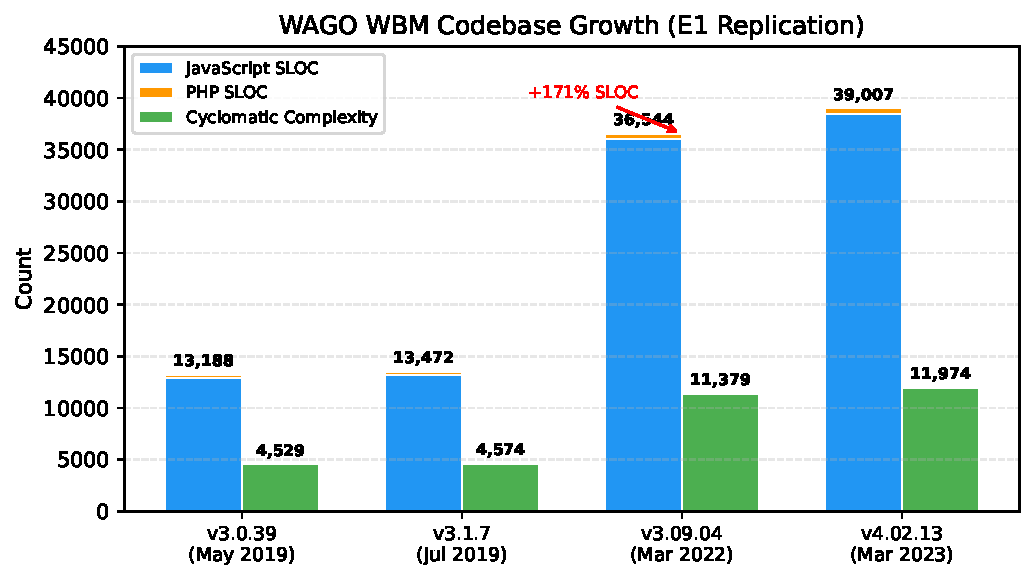
\includegraphics[width=\columnwidth]{e1_sloc_growth.pdf}
\caption{WAGO WBM codebase growth across four firmware versions,
showing total SLOC (stacked JS/PHP) and cyclomatic complexity.}
\label{fig:e1}
\end{figure}

\subsection{Qualitative API Surface Analysis}

This study also provides a qualitative analysis on the updated web-based features from v3.0.39 and v4.02.13, revealing \emph{what kind} of functionality was added. Table~\ref{tab:api-surface} summarizes the new functional categories.

\begin{table}[ht]
\centering
\caption{New JavaScript functional categories in v4.02.13.}
\label{tab:api-surface}
\begin{tabular}{@{}lrl@{}}
\toprule
\textbf{Category} & \textbf{New files} & \textbf{Notable additions} \\
\midrule
Core framework    & 18 & Plugin loader (\texttt{pfc.js}) \\
Security/Auth     & 12 & AIDE IDS, firewall, cert mgmt \\
Industrial proto. & 12 & OPC UA PKI, WDA scan toggle \\
Monitoring        & 12 & Pcap logging, runtime task list \\
Cloud/Remote      &  7 & Azure/AWS/MQTT connectivity \\
Container/Infra   &  4 & Docker management, pkg server \\
API documentation &  1 & OpenAPI self-describing REST \\
\bottomrule
\end{tabular}
\end{table}

The newly added features such as AIDE intrusion detection, firewall configuration, and certificate management are controlled by the smae web interface that the CVE chain can compromise. There is a possiblity of these tools being exploited by an attacker. Meanwhile, Docker on PLCs and persistent MQTT cloud channels may suggest new attack surface that do not exist in the 2019 firmware.

% ---------------------------------------------------------------
% V. Service Worker Resurrection Testbed (E4)
% ---------------------------------------------------------------
\section{Service Worker Resurrection (E4)}
\label{sec:e4}

\subsection{Six-Step Resurrection Cycle}

This study verified all the steps of the malware resurrection cycle stated in Section~IV-C of~\cite{ironspider2024}:

\begin{enumerate}
  \item \textbf{SW registration.} When loading the page for the first time, the browser fetches \texttt{sw.js} and registers it at scope \texttt{/}. Looking at DevTools confirms ``activated and is running.''
  \item \textbf{Payload delivery.} As \texttt{malware.js} is injected, it starts to execute display spoofing (sensor values turn green) and exfiltration simulation for credentials logged to console.
  \item \textbf{Factory reset.} \texttt{malware.js} from the server, simulating a factor reset. The SW remains registered in the browser profile.
  \item \textbf{SW detects absence.} The SW's \texttt{setInterval} fetches for \texttt{/malware.js} within 5 seconds, and receives HTTP~404.
  \item \textbf{Re-upload.} The SW retrieves the payload from\texttt{CacheStorage} and POSTs it to \texttt{/upload} (this is analogous to the original paper's CVE chain).Server log confirms: ``\texttt{RESURRECTION: wrote malware.js}.''
  \item \textbf{Payload re-execution.} The SW sends \texttt{postMessage(\{type:~'RESURRECTED'\})} to all open tabs. Display spoofing resumes with the re-injected malware.
\end{enumerate}

All six steps above executed autonomously wihtin one SW polling interval of 5~seconds. This confirms the paper's claim on malware resurrection after the factory reset.

\subsection{Hardware Replacement Survival}

This study also evaluated the paper's claim that resurrection survives hardware replacement. This was achieved by simulating full server process replacement:

\begin{enumerate}
  \item Record server PID via \texttt{GET /server-info} (PID~3{,}725{,}031).
  \item Kill the Node.js process (\texttt{Ctrl+C}).
  \item Delete \texttt{malware.js} and \texttt{sw.js} from disk.
  \item Restart the server.
  \item Record new PID (3{,}728{,}686) --- different process confirmed.
\end{enumerate}

The browser's SW registration and activation persisted, despite the complete server replacement. The full resurrection cycle was executed within the SW polling interval, re-uploading both the cached \texttt{malware.js} \emph{and} \texttt{sw.js} to the new server instance. This supports the paper's claim that the SW registration resides in the browser, not the physical device.

\subsection{The 24-Hour Cache Limit}

The paper mentions a ``24-hour cache limit'' as a limitation for SW. This study identified two relevant mechanisms in the W3C SW specification~\cite{w3c-sw} to look into this claim further:

\begin{enumerate}
  \item \textbf{SW script update check interval} (\S9.2): the browser fetches the SW script at most once per 24 hours per navigation, and compares it with the registered SW byte-for-byte. 

  \item \textbf{CacheStorage eviction}: the specification does \emph{not} make a 24-hour eviction policy compulsory. Storage entries are evicted only under explicit user action or storage pressure.
\end{enumerate}

This study empirically confirmed that CacheStorage entries persist across browser tab closure, server restarts, and page refreshes. The only reliable solution to eliminate the SW is explicit SW unregistration via DevTools. 
% ---------------------------------------------------------------
% VI. OpenPLC Capability Demonstration
% ---------------------------------------------------------------
\section{OpenPLC Capability Demonstration}
\label{sec:openplc}

This study implemented and confirmed the functionality of the three key IronSpider capabilities depicted in the original paper. This was achieved on OpenPLC Runtime v3 with a custom water pump control program (\texttt{water\_pump.st}).

\subsection{Capability 1: Sensor Spoofing}

The injected malware wraps the response from \texttt{/monitor-update} by gaining access to the DOM update in the monitoring page. The \texttt{ironspiderSpoof()} function parses the HTML table from the API, finds the row containing \texttt{water\_level}, records the actual value to \texttt{localStorage}, and returns a fabricated reading value before display. The operator observes a normal water level when the actual value may be dangerously high.

\subsection{Capability 2: Alarm Suppression via Spoofing}

When the water level exceeds the alarm threshold of 80, the PLC sets \texttt{alarm\_active} to \texttt{TRUE}. The spoofing The spoofing function detects the \texttt{bool\_true.png} indicator and replaces with \texttt{bool\_false.png} in the DOM. The operator is not able to see the actual alarm, potentially ignoring a dangerous situation.

\subsection{Capability 3: Actuator Manipulation}

The malware runs a \texttt{setInterval} loop, calling \texttt{/point-write?value=1\&address=\%QX0.0} every 500\,ms. This changes the actual Boolean value for the pump relay, turning it ON regardless of the ladder logic's output. This bypasses the PLC control loop by using the web API.

While testing for this capability, intermittent toggling of\texttt{pump\_running} between TRUE and FALSE was observed. This is due to the PLC's scan cycle writing the actual, computed value to the same address (\texttt{\%QX0.0}). In a real deployment, combining actuator manipulation while spoofing the pump relay reading would hide the override from the operator entirely.

% ---------------------------------------------------------------
% VII. Behavioral Anomaly Detection
% ---------------------------------------------------------------
\section{Behavioral Anomaly Detection}
\label{sec:detection}

\subsection{Design Rationale for Tier~1}

The paper identifies runtime behavioral detection as an ``open
problem'' because IronSpider uses only legitimate browser APIs
with no syntactically suspicious patterns.
We observe that while the \emph{payload} is indistinguishable from
benign JavaScript, the \emph{delivery mechanism} --- a Service Worker
polling loop --- produces distinguishable HTTP request metadata.

The paper leaves detection of IronSpider as an ``open problem'' since IronSpider uses only legitimate browser API with no suspicious patterns detected by JavaScript analysers. This study observed that while the \emph{payload} itself is indistinguishable from benign JavaScript, the \emph{SW polling loop} for the malware may produce distinguialbe HTTP request metadata useful for detection.

This study focused on detecting SW-originated fetch using two browser-generated headers:

\begin{itemize}
  \item \textbf{\texttt{Sec-Fetch-Dest: empty}.} This header is set for all \texttt{fetch()} API calls according to the W3C Fetch Metadata specification, while a \texttt{<script src>} tag sets \texttt{Sec-Fetch-Dest: script} instead. JavaScript cannot forge or suppress this header.

  \item \textbf{\texttt{Referer} ending in \texttt{.js}.}\texttt{fetch()} calls initiated by SW sets the SW script URL as Referer (e.g., \texttt{/static/sw.js} in OpenPLC's case). Page-originated \texttt{fetch()} calls has the page URL as the value for Referer (e.g., \texttt{/monitoring}), which does not end in \texttt{.js}.

\end{itemize}

Neither signal alone is sufficient: \texttt{Sec-Fetch-Dest: empty}
also matches page-originated \texttt{fetch()} calls (e.g., AJAX
polling in the monitoring page), and a \texttt{.js} Referer could
theoretically appear in benign SW scenarios.
The conjunction of both signals within a sliding window
(3~requests in 90~seconds) identifies the characteristic SW
polling loop.

\subsubsection{Iterative Development}

The final design was reached through two failed iterations:

\begin{enumerate}
  \item \textbf{Count-based (rejected):} counting all GET requests
        to \texttt{/static/malware.js} produced immediate false
        positives because the monitoring page loads the file via
        \texttt{<script src>}.

  \item \textbf{Cache-Control filter (rejected):} the WHATWG Fetch
        specification states that \texttt{cache:~'no-store'} appends
        \texttt{Cache-Control:~no-cache} to the request.
        However, Chromium-based browsers (Chrome, Brave) do \emph{not}
        send this header --- they handle the cache mode internally.
        The \texttt{Cache-Control} header is completely absent from
        SW \texttt{fetch()} requests on these browsers.
\end{enumerate}

A debug header dump revealed \texttt{Sec-Fetch-Dest} and
\texttt{Referer} as the correct discriminators, leading to the
final design.

\subsection{False Positive Evaluation}

We disabled the malware injection (commented out the payload block
in \texttt{pages.py}) and removed \texttt{malware.js} and
\texttt{sw.js} from the server.
The detector ran for five minutes of normal operator interaction
(page loads, monitoring refreshes, manual point writes).
\textbf{Zero Tier~1 alerts} were generated.

Normal browser requests to OpenPLC produce
\texttt{Sec-Fetch-Dest: document} (page loads),
\texttt{Sec-Fetch-Dest: script} (\texttt{<script src>} loads),
or \texttt{Sec-Fetch-Dest: empty} with a non-\texttt{.js} Referer
(AJAX polling from the monitoring page).
None of these combinations match the Tier~1 conjunction.

\subsection{Evasion Evaluation}

We tested three evasion techniques against the Tier~1 detector:

\begin{table}[ht]
\centering
\caption{Evasion techniques against the Tier~1 detector.}
\label{tab:evasion}
\small
\begin{tabular}{@{}lp{3.2cm}c@{}}
\toprule
\textbf{Evasion} & \textbf{Technique} & \textbf{Det.?} \\
\midrule
SW rename        & Rename to \texttt{resurrect.js} & Yes \\
Slow polling     & Interval $\to$ 90\,s & No \\
Referer suppress & \texttt{no-referrer} policy & No \\
\bottomrule
\end{tabular}
\end{table}

\textbf{E1 (SW rename):} The detector is filename-agnostic ---
it checks whether any \texttt{Referer} ends in \texttt{.js},
not a specific filename.
The alert fired correctly after renaming.

\textbf{E2 (slow polling):} With one request per 90 seconds, only
one request accumulates per window, never reaching the threshold
of~3.
\emph{Countermeasure:} reduce the threshold to~1 (any single
SW-context fetch triggers an alert), at the cost of potential false
positives if a benign SW is deployed on the PLC.
Alternatively, extend the window beyond 90 seconds.

\textbf{E3 (Referer suppression):} Adding
\texttt{referrerPolicy:~'no-referrer'} to the fetch options causes
the browser to omit the \texttt{Referer} header entirely.
With no Referer to inspect, Tier~1's second signal is eliminated.
\emph{Countermeasure:} treat the \emph{absence} of a Referer header
on a \texttt{Sec-Fetch-Dest: empty} request as suspicious, since
legitimate page-originated fetch calls always include a Referer
in standard browser configurations.

% ---------------------------------------------------------------
% VIII. Discussion
% ---------------------------------------------------------------
\section{Discussion}
\label{sec:discussion}

\subsection{Replication Fidelity}

Our E1 results reproduce the paper's SLOC and complexity figures
within rounding error, validating the measurement methodology.
The intermediate firmware versions provide new evidence that the
codebase expansion was gradual, driven primarily by the v3.1.7 $\to$
v3.09.04 transition (2019--2022), which added the plugin
architecture, cloud connectivity, and Docker support.

The E4 testbed successfully replicates all six resurrection steps
and provides the first empirical confirmation of the hardware
replacement survival claim.
Our clarification of the ``24-hour cache limit'' as the SW update
check interval (not CacheStorage eviction) resolves an ambiguity
in the original paper.

\subsection{Limitations}

\textbf{OpenPLC adaptation.}
The most significant limitation is the absence of a CVE-based
delivery vector on OpenPLC.
Our manual injection simulates the \emph{effect} of the exploit
chain but does not validate the \emph{delivery} phase.
The SW scope is also confined to \texttt{/static/} rather than
\texttt{/}, which limits the SW's ability to intercept all page
fetches.

\textbf{Single browser tested.}
The detector's Tier~1 signals (\texttt{Sec-Fetch-Dest} and
\texttt{Referer} behavior) were validated on Brave (Chromium-based).
Firefox and Safari may set these headers differently;
cross-browser validation is left for future work.

\textbf{False positive test scope.}
Five minutes of normal operation is a limited evaluation.
A production deployment would require multi-day testing across
multiple operator workflows and network conditions.

\textbf{Tier~2 and Tier~3 not rigorously evaluated.}
We focused evaluation effort on Tier~1 as the primary contribution.
Tier~2 (write rate) and Tier~3 (read-write latency) were implemented
and observed to fire during attack scenarios but were not subjected
to systematic false positive testing.

\subsection{Implications for ICS Defense}

The detection gap identified by the paper is real but not
insurmountable.
Server-side behavioral detection using browser-generated Fetch
Metadata headers offers a practical defense layer that requires
no client-side instrumentation and no modification to the browser.
The approach is deployable as a lightweight WAF module, consistent
with the ``PLC-configured WAF'' countermeasure proposed in
Table~VII of~\cite{ironspider2024}.

The evasion analysis reveals that the Referer header is the weaker
of the two signals.
A more robust design would combine Tier~1 with Content Security
Policy (CSP) headers that restrict SW registration, or with
Subresource Integrity (SRI) checks on served JavaScript files.

% ---------------------------------------------------------------
% IX. Conclusion
% ---------------------------------------------------------------
\section{Conclusion}
\label{sec:conclusion}

We replicated key experiments from the IronSpider web-based PLC
malware study, confirming the paper's firmware growth analysis,
the full six-step SW resurrection cycle including hardware replacement
survival, and the three core attack capabilities on an alternative
PLC platform (OpenPLC).
We clarified the ``24-hour cache limit'' as the SW script update
check interval, not a CacheStorage eviction policy, providing a
more precise characterization of the persistence window.

To address the paper's stated detection gap, we implemented a
three-tier behavioral detector.
Tier~1 achieves zero false positives by correlating two
browser-generated headers (\texttt{Sec-Fetch-Dest: empty} and
a \texttt{.js}-suffixed \texttt{Referer}) to identify SW polling
loops.
Two of three tested evasion techniques defeat Tier~1, but both
have straightforward countermeasures: extending the detection
window and treating absent Referer headers as suspicious.

Future work includes cross-browser validation of the Fetch Metadata
signals, integration with CSP-based SW registration restrictions,
and multi-day false positive evaluation in a production-representative
ICS environment.

% ---------------------------------------------------------------
% References
% ---------------------------------------------------------------
\begin{thebibliography}{9}

\bibitem{ironspider2024}
D.~Pickren, T.~Shekari, S.~Zonouz, and R.~Beyah,
``Compromising Industrial Processes using Web-Based PLC Malware,''
in \emph{Proc. NDSS}, 2024.
DOI: 10.14722/ndss.2024.23049.

\bibitem{stuxnet}
N.~Falliere, L.~O.~Murchu, and E.~Chien,
``W32.Stuxnet Dossier,''
Symantec Security Response, Feb. 2011.

\bibitem{harvey2017}
L.~Garcia, F.~Brasser, M.~H.~Cintuglu, A.-R.~Sadeghi, O.~Mohammed,
and S.~A.~Zonouz,
``Hey, My Malware Knows Physics! Attacking PLCs with Physical Model Aware Rootkit,''
in \emph{Proc. NDSS}, 2017.

\bibitem{w3c-sw}
A.~Russell et al., ``Service Workers 1,''
W3C Recommendation, Nov. 2022.
\url{https://www.w3.org/TR/service-workers/}

\bibitem{openplc}
T.~Alves and J.~Morris,
``OpenPLC: An Open Source Alternative to Automation,''
in \emph{Proc. IEEE SmartComp}, 2014.

\bibitem{cujo}
L.~Canali, M.~Cova, G.~Vigna, and C.~Kruegel,
``Prophiler: A Fast Filter for the Large-Scale Detection of Malicious Web Pages,''
in \emph{Proc. WWW}, 2011.

\bibitem{zozzle}
C.~Curtsinger, B.~Livshits, B.~Zorn, and C.~Seifert,
``ZOZZLE: Fast and Precise In-Browser JavaScript Malware Detection,''
in \emph{Proc. USENIX Security}, 2011.

\bibitem{jast}
S.~Fass, M.~Backes, and B.~Stock,
``JaSt: Fully Syntactic Detection of Malicious (Obfuscated) JavaScript,''
in \emph{Proc. DIMVA}, 2018.

\bibitem{jstap}
S.~Fass, M.~Backes, and B.~Stock,
``JStap: A Static Pre-Filter for Malicious JavaScript Detection,''
in \emph{Proc. ACSAC}, 2019.

\end{thebibliography}

\end{document}
